\section{Implementación}

\subsection{Estructura del Proyecto Backend}

El backend está organizado en \textbf{3 módulos principales} siguiendo el principio de separación de responsabilidades:

\subsubsection{Módulo 1: Security (Seguridad)}

Responsable de autenticación, autorización y gestión de usuarios:

\begin{itemize}
    \item \textbf{Modelos}: Person, User, Role, Permission, Form, Module, DocumentType, RoleFormPermission, FormModule
    \item \textbf{10 Repositorios}: Acceso a datos de usuarios, roles, permisos
    \item \textbf{15 Servicios}: Lógica de autenticación 2FA, recuperación de contraseña, gestión de roles
    \item \textbf{12 ViewSets}: Endpoints de API REST
    \item \textbf{Funcionalidades clave}:
    \begin{itemize}
        \item Autenticación de dos factores (2FA) por correo
        \item JWT (JSON Web Tokens) para sesiones
        \item Sistema de permisos granular (Rol → Formulario → Permiso)
        \item Recuperación de contraseña con códigos temporales
        \item Middleware de autenticación JWT
    \end{itemize}
\end{itemize}

\subsubsection{Módulo 2: General (Datos Maestros)}

Gestiona entidades generales del sistema:

\begin{itemize}
    \item \textbf{Modelos}: Regional, Center, Sede, Program, Ficha, Apprentice, Instructor, KnowledgeArea, TypeContract, Notification, LegalDocument, SupportContact
    \item \textbf{17 Repositorios}: Uno por cada entidad
    \item \textbf{17 Servicios}: Lógica de negocio específica
    \item \textbf{18 ViewSets}: Endpoints CRUD completos
    \item \textbf{Funcionalidades clave}:
    \begin{itemize}
        \item Gestión jerárquica: Regional → Centro → Sede
        \item Control de instructores (límite de aprendices, contratos)
        \item Sistema de notificaciones con WebSockets (Django Channels)
        \item Gestión de documentos legales y soporte técnico
        \item Tareas asíncronas con Celery (desactivación automática de instructores)
    \end{itemize}
\end{itemize}

\subsubsection{Módulo 3: Assign (Asignaciones)}

Núcleo del sistema, gestiona todo el proceso de asignación:

\begin{itemize}
    \item \textbf{Modelos}: RequestAsignation, AsignationInstructor, VisitFollowing, Message, Enterprise, Boss, HumanTalent, ModalityProductiveStage, AsignationInstructorHistory
    \item \textbf{10 Repositorios}: Acceso a datos de solicitudes, asignaciones, visitas
    \item \textbf{10 Servicios}: Lógica compleja de asignación y seguimiento
    \item \textbf{10 ViewSets}: Endpoints especializados
    \item \textbf{Funcionalidades clave}:
    \begin{itemize}
        \item Flujo completo: Solicitud → Asignación → Visitas → Valoración
        \item Estados de solicitud: SIN\_ASIGNAR, ASIGNADO, VERIFICANDO, PRE-APROBADO, RECHAZADO, FINALIZADA
        \item Generación automática de 3 visitas (Concertación, Parcial, Final)
        \item Sistema de mensajes entre instructor y coordinador
        \item Historial completo de reasignaciones
        \item Envío automático de correos (Celery tasks)
        \item Generación de PDFs de solicitudes
    \end{itemize}
\end{itemize}

\textbf{Estructura de cada módulo}:

\begin{itemize}
    \item \textbf{apps/[module\_name]/}
    \begin{itemize}
        \item \textbf{entity/}: Modelos, serializers y enums (10-18 modelos por módulo)
        \item \textbf{repositories/}: Acceso a datos (uno por cada entidad)
        \item \textbf{services/}: Lógica de negocio
        \item \textbf{views/}: ViewSets con endpoints de API
        \item \textbf{emails/}: Clases para envío de correos
        \item \textbf{templates/}: HTML para correos
        \item \textbf{migrations/}: Migraciones de base de datos
        \item \textbf{urls.py}: Rutas del módulo
    \end{itemize}
\end{itemize}

\textbf{Ventajas de esta arquitectura}:
\begin{itemize}
    \item \textbf{Modularidad}: Cada módulo es independiente y puede desarrollarse en paralelo
    \item \textbf{Escalabilidad}: Fácil agregar nuevos módulos sin afectar los existentes
    \item \textbf{Mantenibilidad}: Código organizado por dominio de negocio
    \item \textbf{Reutilización}: Repositorios y servicios base heredables
    \item \textbf{Testing}: Cada capa se puede testear independientemente
\end{itemize}

\subsection{Estructura del Proyecto Frontend}

El frontend sigue una arquitectura por capas con React y TypeScript, totalmente tipado:

\subsubsection{Capa de Configuración y Servicios (src/Api/)}

\begin{itemize}
    \item \textbf{config/ConfigApi.ts}: Centraliza todos los endpoints del backend (más de 100 endpoints)
    \item \textbf{Services/} (32 archivos): Funciones especializadas para cada entidad
    \begin{itemize}
        \item Ejemplo: \texttt{User.ts}, \texttt{RequestAssignaton.ts}, \texttt{Instructor.ts}
        \item Cada servicio maneja peticiones HTTP (GET, POST, PUT, DELETE, PATCH)
        \item Incluye manejo de errores y parsing de respuestas
    \end{itemize}
    \item \textbf{types/}: Interfaces TypeScript fuertemente tipadas
    \begin{itemize}
        \item \texttt{entities/}: 14 interfaces de entidades (User, Instructor, RequestAsignation, etc.)
        \item \texttt{Modules/}: 2 interfaces de módulos complejos
    \end{itemize}
\end{itemize}

\subsubsection{Capa de Componentes (src/components/)}

Componentes React organizados por funcionalidad:

\begin{itemize}
    \item \textbf{assing/}: 8 componentes para asignaciones (ModalAssign, AssignTableView, etc.)
    \item \textbf{ApplicationEvaluation/}: Evaluación de solicitudes por coordinador
    \item \textbf{ModuleSecurity/}: 28 componentes para roles, permisos, usuarios
    \item \textbf{Dashboard/}: 6 componentes de tableros (Admin, Instructor, Aprendiz)
    \item \textbf{Login/}: 11 componentes de autenticación (2FA, recuperación, registro)
    \item \textbf{MainLayout/}: 7 componentes de estructura (Navbar, Sidebar, Footer)
    \item \textbf{ui/}: 49 componentes reutilizables (botones, modales, formularios - Radix UI)
    \item \textbf{Componentes genéricos}: FilterBar, Paginator, ConfirmModal, LoadingOverlay, etc.
\end{itemize}

\subsubsection{Capa de Lógica (src/hook/)}

Custom hooks que encapsulan lógica reutilizable (24 hooks):

\begin{itemize}
    \item \texttt{useForms.ts}: Gestión de formularios del sistema
    \item \texttt{useRoles.tsx}: Lógica de roles y permisos
    \item \texttt{useInstructorAssignments.ts}: Asignaciones de instructor
    \item \texttt{useRequestAssignation.ts}: Solicitudes de asignación
    \item \texttt{useNotification.ts}: Sistema de notificaciones en tiempo real
    \item \texttt{use-password-reset.ts}: Recuperación de contraseña
    \item \texttt{useApprenticeDashboard.ts}: Tablero del aprendiz
    \item \texttt{useGenericFilter.ts}: Filtros reutilizables
\end{itemize}

\subsubsection{Capa de Presentación (src/pages/)}

Páginas principales de la aplicación (15 páginas):

\begin{itemize}
    \item \texttt{Index.tsx}: Login y autenticación
    \item \texttt{Home.tsx}: Dashboard según rol
    \item \texttt{Assign.tsx}: Asignación de instructores
    \item \texttt{ApplicationEvaluation.tsx}: Evaluación de solicitudes
    \item \texttt{Following.tsx}: Seguimiento de visitas
    \item \texttt{RegisterEP.tsx}: Registro de solicitud de etapa productiva
    \item \texttt{Admin.tsx}: Panel de administración
    \item \texttt{Perfil.tsx}: Perfil de usuario
\end{itemize}

\textbf{Ventajas de esta arquitectura frontend}:
\begin{itemize}
    \item \textbf{Tipado completo}: TypeScript previene errores en tiempo de compilación
    \item \textbf{Reutilización}: Componentes y hooks reutilizables
    \item \textbf{Separación de responsabilidades}: Lógica separada de presentación
    \item \textbf{Mantenibilidad}: Fácil localizar y modificar funcionalidades
    \item \textbf{Testing}: Hooks y componentes testeables independientemente (Jest + React Testing Library)
\end{itemize}

\subsection{Flujo de una Petición}

Cuando un usuario hace una petición, el flujo es el siguiente:

\begin{enumerate}
    \item Cliente (React) hace petición HTTP
    \item Django recibe en ViewSet
    \item ViewSet valida con Serializer
    \item ViewSet llama al Service
    \item Service ejecuta lógica de negocio
    \item Service usa Repository para datos
    \item Repository consulta el Model/BD
    \item Respuesta sube por las capas
    \item ViewSet serializa respuesta
    \item Cliente recibe JSON
\end{enumerate}

\subsection{Ejemplo Práctico: Crear Tipo de Contrato}

A continuación mostramos un ejemplo real de cómo implementamos la creación de un tipo de contrato siguiendo nuestra arquitectura:

\textbf{1. ViewSet (recibe petición):}

\ifminted
\begin{minted}[linenos,fontsize=\small]{python}
def create(self, request, *args, **kwargs):
    service = self.service_class()
    instance, error = service.create_type_contract(
        request.data
    )
    if error:
        return Response(
            {"detail": error}, 
            status=400
        )
    serializer = self.get_serializer(instance)
    return Response(
        serializer.data, 
        status=201
    )
\end{minted}
\else
\begin{lstlisting}[language=Python,basicstyle=\small]
def create(self, request, *args, **kwargs):
    service = self.service_class()
    instance, error = service.create_type_contract(
        request.data
    )
    if error:
        return Response(
            {"detail": error}, 
            status=400
        )
    serializer = self.get_serializer(instance)
    return Response(
        serializer.data, 
        status=201
    )
\end{lstlisting}
\fi

\textbf{2. Service (lógica de negocio):}

\ifminted
\begin{minted}[linenos,fontsize=\small]{python}
def create_type_contract(self, validated_data):
    name = validated_data.get('name', '').strip()
    if not name:
        return None, "El nombre es requerido."
    
    # Verificar duplicados
    exists = TypeContract.objects.filter(
        name__iexact=name, 
        delete_at__isnull=True
    ).exists()
    
    if exists:
        return None, "Ya existe ese contrato."
    
    serializer = TypeContractSerializer(
        data=validated_data
    )
    if serializer.is_valid():
        instance = serializer.save()
        return instance, None
    return None, serializer.errors
\end{minted}
\else
\begin{lstlisting}[language=Python,basicstyle=\small]
def create_type_contract(self, validated_data):
    name = validated_data.get('name', '').strip()
    if not name:
        return None, "El nombre es requerido."
    
    # Verificar duplicados
    exists = TypeContract.objects.filter(
        name__iexact=name, 
        delete_at__isnull=True
    ).exists()
    
    if exists:
        return None, "Ya existe ese contrato."
    
    serializer = TypeContractSerializer(
        data=validated_data
    )
    if serializer.is_valid():
        instance = serializer.save()
        return instance, None
    return None, serializer.errors
\end{lstlisting}
\fi

\subsection{Custom Hooks en React}

Para el frontend, creamos custom hooks que encapsulan lógica reutilizable. Estos hooks nos permiten:
\begin{itemize}
    \item Reutilizar lógica en múltiples componentes
    \item Mantener el código limpio
    \item Facilitar el testing
    \item Separar lógica de presentación
\end{itemize}

\subsection{Comparación Antes/Después}

La Figura~\ref{fig:comparacion_codigo} muestra la diferencia clara entre nuestro código antes y después de aplicar los patrones:

\begin{figure}[htbp]
    \centering
    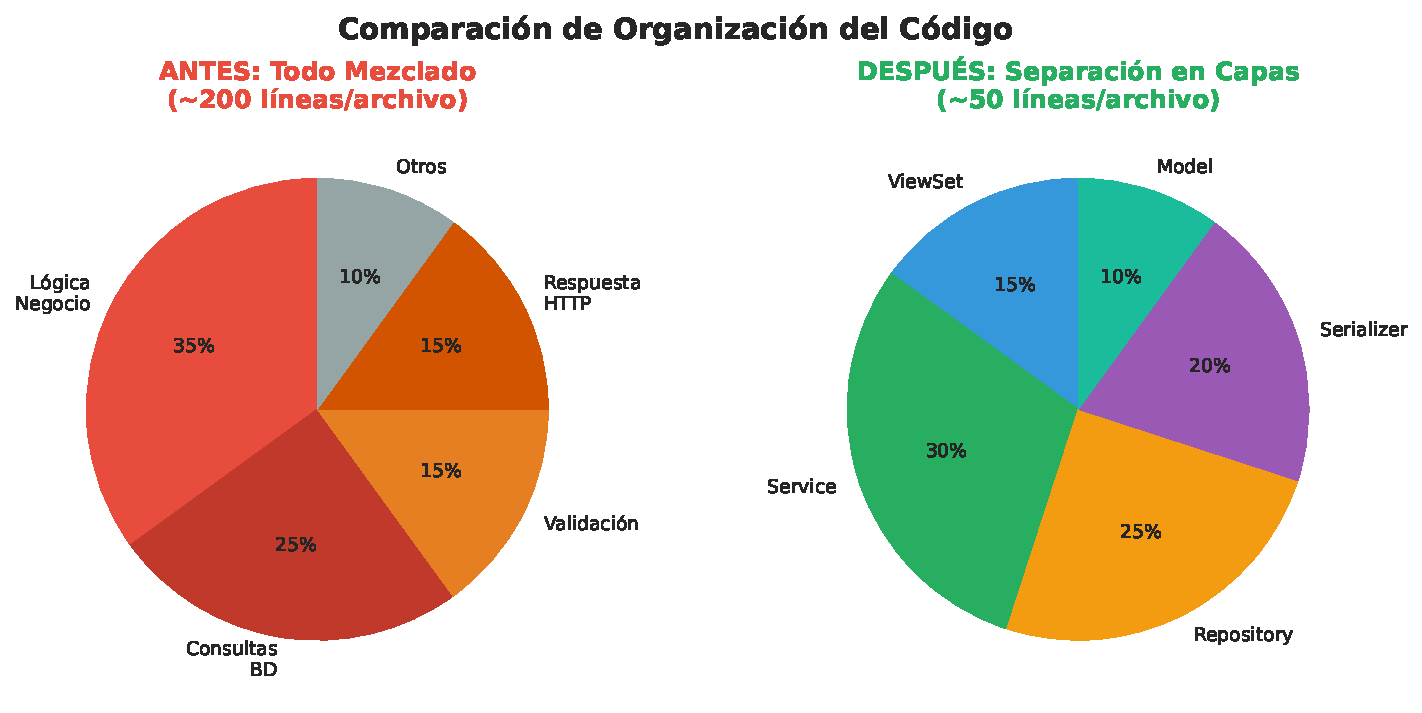
\includegraphics[width=0.48\textwidth]{graphics/comparacion_codigo.pdf}
    \caption{Comparación de complejidad del código antes y después de aplicar patrones}
    \label{fig:comparacion_codigo}
\end{figure}

\textbf{Antes}: Todo mezclado en la vista (validación, consulta a BD, lógica de negocio, respuesta).

\textbf{Después}: ViewSet limpio que solo coordina, Service con lógica de negocio, Repository con acceso a datos.

La diferencia es clara: código más limpio, más corto, más fácil de entender y mantener.
